\documentclass[fleqn,utf8,aspectratio=169,14pt]{beamer}
%\documentclass[fleqn,utf8,aspectratio=169,14pt,handout]{beamer}

\usepackage{url}
\usepackage{tabto}
\usepackage{dutchcal}
\usepackage{setspace}
\usepackage{xfrac}
\usefonttheme{serif}
\usepackage{graphicx}
\usepackage{listing}
\usepackage{listings}
\usepackage{xcolor}

\lstset{
	basicstyle=\ttfamily\footnotesize,
	keywordstyle=\color{blue},
	commentstyle=\color{gray},
	stringstyle=\color{red},
	numbers=left,
	numberstyle=\tiny,
	stepnumber=1,
	numbersep=8pt,
	frame=single,
	breaklines=true,
	showstringspaces=false,
	tabsize=4,
	language=Python
}

\title{Tutorial do VSCode}
\author{Python para Todos}
\date{\today}

\graphicspath{{./figs/}}
\makeatletter
\def\input@path{{./figs/}}
\makeatother

\newcommand{\AddTeXFigure}[2]
{
	\begin{frame}{#1}
		\null
		\vspace*{-5mm}
		\hspace*{-10mm}
		\input{#2}
	\end{frame}
}
\begin{document}
	

	\begin{frame}
		\titlepage
	\end{frame}
	

	\begin{frame}{Sumário}
		\tableofcontents
	\end{frame}
	

	\section{Introdução}
	\begin{frame}{Introdução}
		O Visual Studio Code (VSCode) é um editor de código gratuito da Microsoft, rápido e personalizável, com:
		\begin{itemize}
			\item Destaque de sintaxe e autocompletar
			\item Extensões para várias linguagens (Python, JavaScript, etc.)
			\item Suporte a Git
			\item Interface moderna
		\end{itemize}
		Ideal para programadores de todos os níveis.
	\end{frame}
	
	\section{Como definir o tipo de um arquivo?}
	\begin{frame}{Como definir o tipo de um arquivo?}
		Para fazer isso no VSCode basta após inserir o nome do arquivo digitar "." seguido do seu tipo.\\
		Exemplo com o arquivo de nome "teste" em Python:\\
		
			\centering  Nome do arquivo: teste.py
	\end{frame}

	\section{Criando um arquivo}
	\begin{frame}{Criando um arquivo}
		Primeiro passo:
		Clicar em "File", no canto superior esquerdo, e em seguida em "New File ..."
		\centering 
		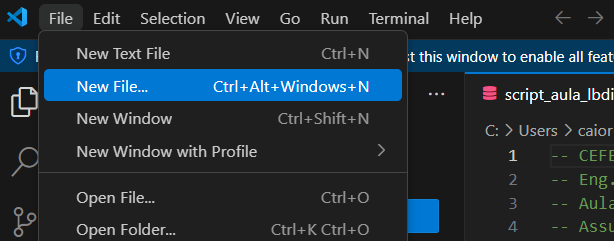
\includegraphics[width=0.8\textwidth]{Imagem1.png}
	\end{frame}
	
	\begin{frame}{Criando um arquivo}
		Segundo passo:
		Definir o nome do arquivo como "teste.py"
		\centering % Centraliza a imagem
		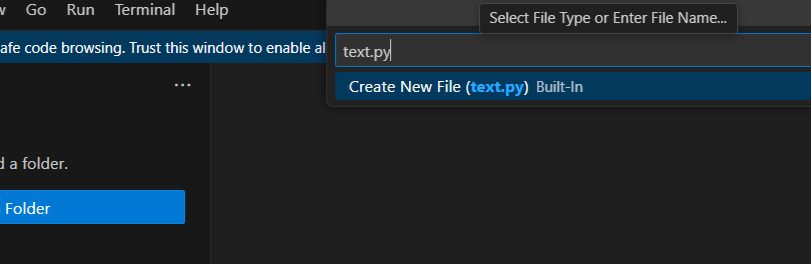
\includegraphics[width=0.8\textwidth]{Imagem2.png}
	\end{frame}
	
	\section{Executando o arquivo}
	\begin{frame}{Executando o arquivo}
		Digitar print("Hello World!")
		E em seguida vamos executar o código, clicando em Run Python File, no canto superior direito
		\centering % Centraliza a imagem
		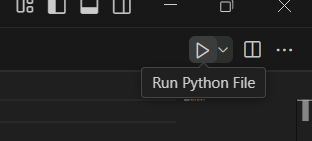
\includegraphics[width=0.8\textwidth]{Imagem3.png}
	\end{frame}
	
	
	\begin{frame}{Executando o arquivo}
		\centering % Centraliza a imagem
		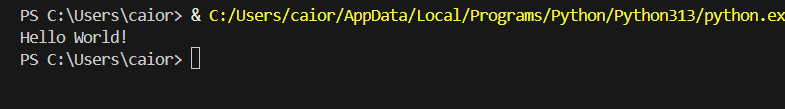
\includegraphics[width=1.2\textwidth]{Imagem4.png}
	\end{frame}
	
	\section{O que é o Pygame?}
	\begin{frame}{O que é o Pygame?}
		O PyGame é uma biblioteca do Python para criação de jogos 2D, permitindo:
		\begin{figure}
			\centering
			
\includegraphics[width=0.7\linewidth]{Imagem5}
			\label{fig:imagem5}
		\end{figure}
		
		\begin{itemize}
			\item Criar movimentação para personagens
			\item Gerar cenário
			\item Colocar música
			\item Colocar Sprites para os personagens
		\end{itemize}
		
	\end{frame}
	
	\section{Vantagens do Pygame}
	\begin{frame}{Vantagens do Pygame}
		
		\begin{itemize}
			\item Simples de aprender (utiliza Python)
			\item Não é uma Game Engine pesada para rodar
			\item Porta de entrada para outras plataformas de criação de jogos, como:
			\begin{itemize}
				\item \textbf{Godot} (utiliza uma linguagem semelhante à Python)
				\item \textbf{Unreal Engine}
				\item \textbf{Game Maker Studio}
			\end{itemize}
		\end{itemize}
		
	\end{frame}
	
	\section{O que iremos criar nesse curso?}
	\begin{frame}{O que iremos criar nesse curso?}
		
		Nesse curso, iremos criar dois jogos simples:
		
		\begin{itemize}
			\item \textbf{Snake (Jogo da cobrinha)}: O clássico jogo da cobrinha em que você deve coletar maçãs que aparecem aleatoriamente no mapa
			\begin{figure}
				\centering
				\includegraphics[width=0.3\linewidth]{"Imagem 6"}
				\label{fig:imagem-6}
			\end{figure}
		\end{itemize}
		
	\end{frame}
	
	\begin{frame}{O que iremos criar nesse curso?}
		
		\begin{itemize}
			\item \textbf{Brick Breaker}: O jogo em que você arremessa uma bola em tijolos para quebrá-los. Toda vez que um bloco é quebrado, a velocidade do jogo aumenta
			\begin{figure}
				\centering
				\includegraphics[width=0.3\linewidth]{"Imagem7"}
				\label{fig:imagem-7}
			\end{figure}
		\end{itemize}
		
	\end{frame}
	
	
	\section{Uma breve visão do Pygame}
	\begin{frame}{Uma breve visão do Pygame}
		Vamos mostrar alguns comandos básicos de Pygame
		\begin{itemize}
			\item \textbf{import pygame as pg} : importa a bilbioteca do pygame. O final "as pg" significa que estamos dando um sobrenome "pg" para o pygame para facilitar a escrita
			\item \textbf{pg.init() e pg.quit()}: inicializa e fecha o pygame
			\item \textbf{tela = pg.display.set\_mode((largura, altura))}: cria a tela do pygame, dado um tamanho de largura e altura
			\item \textbf{clock = pg.time.Clock() e clock.tick(fps)}: define uma variável para ser o clock (tempo de atualização de cada tela do jogo) e quantas vezes por segundo será atualizado a tela
		\end{itemize}
	
		
	\end{frame}
	\begin{frame}{Uma breve visão do Pygame}
		\begin{itemize}
			\item \textbf{pg.key.get\_pressed()} : Pega a tecla digitada pelo usuário no momento (usada para definir a movimentação do personagem)
			\item \textbf{pg.draw.rect(tela, COR, (x, y, largura, altura))}: cria um objeto retangular, que ficará na tela, com uma determinada cor, terá um posição (coordenada) específica e um tamanho (largura e altura)
			\item \textbf{pygame.draw.circle(tela, COR, (x, y), raio)}: cria um círculo, que ficará na tela, com uma determinada cor, terá uma posição específica e um raio
			\item \textbf{pg.display.update()}: atualiza a tela baseado no clock
		\end{itemize}
	\end{frame}
	
	
	\begin{frame}[fragile]{Uma breve visão do Pygame}
		\begin{lstlisting}
import pygame as pg # importa a biblioteca do pygame
		
pg.init() # Inicializa o Pygame
	
largura, altura = 800, 600 # Tamanho da janela
tela = pg.display.set_mode((largura, altura)) #define o tamanho da tela
pg.display.set_caption("Teste") #Coloca uma legenda para a tela
	
x, y = 100,100 #define a posição inicial do jogador		
velocidade = 5 #vai definir a velocidade do personagem mexendo na tela
clock = pg.time.Clock() #cria a variável do clock do jogo
		\end{lstlisting}
	\end{frame}
	
	\begin{frame}[fragile]{Uma breve visão do Pygame}
		\begin{lstlisting}
while True:
	clock.tick(60)  # 60 FPS
	tela.fill('white') #preenche o fundo com a cor branca
	for evento in pg.event.get():
		if evento.type == pg.QUIT: #caso o jogo foi fechado
			pg.quit()
	teclas = pg.key.get_pressed() #pega tecla digitada
	if teclas[pg.K_a]:
		x -= velocidade #diminui a posicao do x
	if teclas[pg.K_d]:
		x += velocidade #aumenta a posicao do x
	if teclas[pg.K_w]:
		y -= velocidade #diminui a posicao do y
	if teclas[pg.K_s]:
		y += velocidade #aumenta a posicao do y
	pg.draw.rect(tela,'red',(x, y, 50, 50))
	pg.display.update() #atualiza a tela	
		\end{lstlisting}
	\end{frame}
	
	\begin{frame}{Uma breve visão do Pygame}
		Teremos algo assim:
		
		\begin{figure}
			\centering
			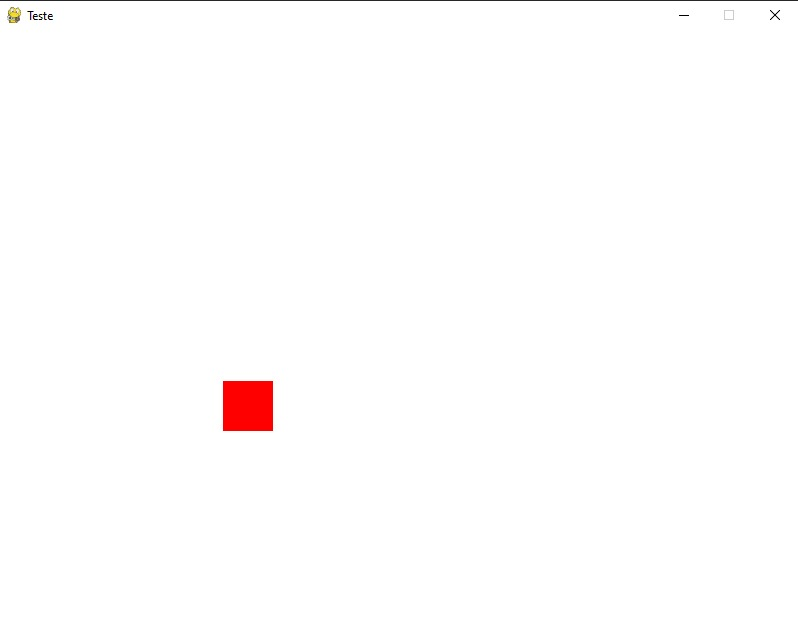
\includegraphics[width=0.7\linewidth]{Imagem8}
			\caption{}
			\label{fig:imagem8}
		\end{figure}
		
	\end{frame}
	
	\section{Criando o jogo da cobrinha}
	\begin{frame}[fragile]{Criando o jogo da cobrinha (SETUP)}
		
		\begin{lstlisting}
import pygame as pg
import random as rd
pg.init()
largura, altura = 720, 720
tela = pg.display.set_mode((largura, altura))
clock = pg.time.Clock()

		\end{lstlisting}
	\end{frame}
	
	\begin{frame}[fragile]{Criando o jogo da cobrinha (SETUP)}
		
		\begin{lstlisting}
velocidade = 5 #define a velocidade(pixel por movimento) do jogo
tamanho_cobra = 15  #define quantos quadrados nossa cobra tera inicialmente
initial_control = pg.Vector2(velocidade,0)
tam = 30 # valor do tamanho dos objetos
cobra_pos = pg.Vector2(tela.get_width()/2, tela.get_height()/2)
maca_pos = pg.Vector2(rd.randint(tam, largura-tam), rd.randint(tam, altura-tam))
control_pos = pg.Vector2(velocidade,0) # será o valor que irá controlar a posicao da maca
lista_cobra = [] #sera a lista que ficara a cobra
		\end{lstlisting}
	\end{frame}
	
	\begin{frame}[fragile]{Criando o evento de parada e os objetos principais}
		\begin{lstlisting}
while True:   
	clock.tick(60)
	tela.fill('white')
	
	for event in pg.event.get():
		if event.type == pg.QUIT:
			pg.quit()
	
	cobra = pg.draw.rect(tela, 'green',(cobra_pos.x, cobra_pos.y, tam, tam))
	maca = pg.draw.rect(tela, 'red',(maca_pos.x, maca_pos.y, tam, tam))
		\end{lstlisting}
	\end{frame}
	
	\begin{frame}[fragile]{Movimentação da cobra}
		\begin{lstlisting}
	key = pg.key.get_pressed()
	if key[pg.K_w]:
		control_pos.y = -velocidade #define o valor e a direcao que a cobra vai andar
		control_pos.x = 0
	if key[pg.K_s]:
		control_pos.y = velocidade
		control_pos.x = 0
	if key[pg.K_a]:
		control_pos.y = 0
		control_pos.x = -velocidade
	if key[pg.K_d]:
		control_pos.y = 0
		control_pos.x = velocidade
	# Muda os valores de posicao da cobra
	cobra_pos.x += control_pos.x 
	cobra_pos.y += control_pos.y
		\end{lstlisting}
	\end{frame}
	
	\begin{frame}[fragile]{Criação da cobra e reconhecendo colisão}
		\begin{lstlisting}
	#Atualização do corpo da cobra
	lista_cabeca = []
	lista_cabeca.append(cobra_pos.x)
	lista_cabeca.append(cobra_pos.y)
	lista_cobra.append(lista_cabeca)
	#Limita o tamanho da cobra
	if len(lista_cobra) > tamanho_cobra:
		del lista_cobra[0]
	for pos in lista_cobra: #desenha a cobra
		pg.draw.rect(tela, 'green', (pos[0], pos[1], tam, tam))
	#Colisao
	if maca.colliderect(cobra):
		maca_pos.x=rd.randint(tam, largura-tam)
		maca_pos.y=rd.randint(tam, altura-tam)
	pg.display.update()
		\end{lstlisting}
	\end{frame}
	
\end{document}}